\chapter{METHODOLOGY}
\section{Overview}
The project follows an iterative prototype-development methodology. Meter telemetry is generated by an ESP32/Wokwi node, validated and processed by a FastAPI backend, recorded in SQLite, and connected to a local Hardhat smart contract for prepaid deduction. The backend returns a control command to the firmware, and the React dashboard reads the resulting system state. Historical seed data is used to initialize and evaluate the remaining-time estimator.
\section{Proposed Block Diagram}
\begin{figure}[ht!]
    \centering
    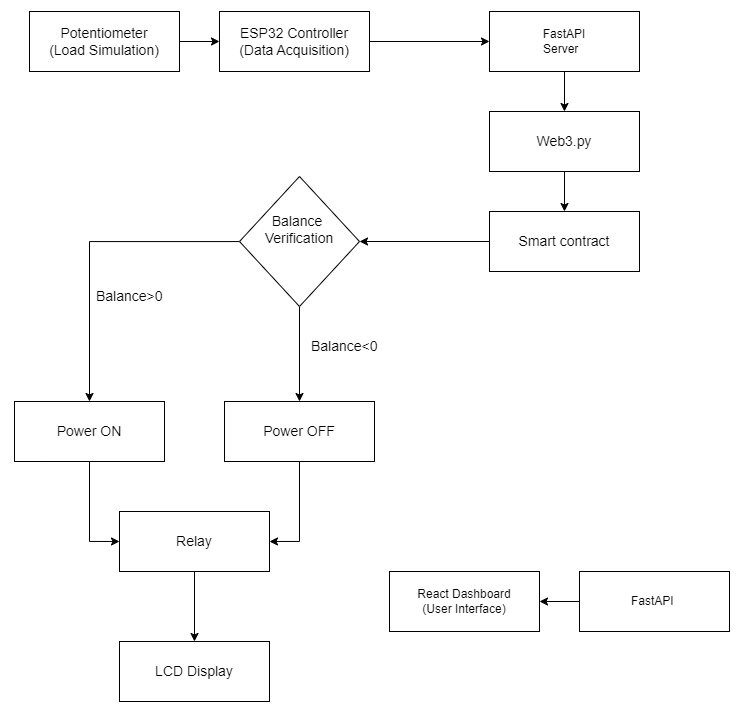
\includegraphics[width=0.8\textwidth]{Graphics/Image 1.png}
    \caption*{Figure-1: Proposed Block Diagram of decentralized power grid.\cite{ref4}}
    \label{fig:blockdiagram}

\end{figure}

\section{System Design}
The architecture is organized into four cooperating layers: the firmware layer for sensing and relay control, the backend layer for validation and orchestration, the blockchain layer for prepaid credit, and the dashboard layer for monitoring. SQLite stores local operational records without replacing the blockchain as the credit ledger.
\begin{figure}[h!]
    \centering
    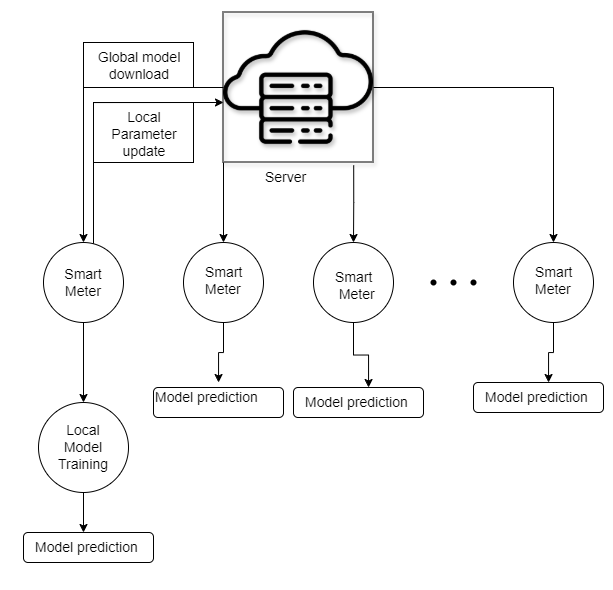
\includegraphics[width=0.8\textwidth]{Graphics/architecture.png}
    \caption*{Figure-2: System Design for decentralized power grid. \cite{ref5}}
    \label{fig:architecurediagram}
\end{figure}
\section{Tools and Techniques}
\begin{itemize}
\item Hardware and simulation: ESP32, current/load sensors, relay, and Wokwi

\item Software: PlatformIO/C++, FastAPI and Web3.py (Python), Hardhat and Solidity, React/Vite, SQLite, and scikit-learn
\end{itemize}



\section{Data Sources}
\subsection{Primary Sources}
Real-time prototype telemetry will be generated by the ESP32/Wokwi edge node. Test scenarios will include normal load, depleted credit, and tamper conditions produced through controlled sensor inputs.
\subsection{Synthetic Data (Machine Learning Training)}
The regression estimator will use the seeded Dharan meter history stored in CSV format. The dataset contains timestamped consumption and remaining-token values, from which time-of-day and day-of-week features are derived. Tamper detection will be evaluated using controlled line/neutral current differences and explicit tamper flags.

\section{Implementation}
\subsection{Hardware Layer Implementation}
The physical edge node is built around an ESP32 configured with PlatformIO. The firmware samples the meter inputs, constructs a JSON telemetry packet, sends it at a fixed interval, and uses the backend response to keep the relay active or isolate the circuit.
\subsection{Blockchain Ledger Implementation}
The transaction layer relies on a Solidity smart contract compiled and tested with Hardhat. The contract maps meter wallets to prepaid credits and exposes balance, funding, deduction, and zero-balance checks. For each accepted reading, the prototype applies a bounded integer deduction based on reported energy and returns the updated balance and isolation decision. Conceptually, the deduction is: \cite{ref6}$$\text{Bal}_{\text{new}} = \text{Bal}_{\text{current}} - \text{Cost}(\text{energy})$$
\subsection{Backend Middleware and ML Integration}
The coordination hub is built with FastAPI. It verifies the meter against SQLite, handles tamper and balance conditions, calls the contract through Web3.py, stores meter history, and returns a relay command. The ML module fits a linear regression baseline for service-time estimation, while current-differential classification provides the tamper flag.\cite{ref7}

\section{Testing and Evaluation}
Testing will be performed at unit, integration, and demonstration levels. Unit tests will verify balance arithmetic, meter validation, current-differential classification, and remaining-time calculations. Integration tests will exercise the telemetry-to-contract-to-relay response flow using a local Hardhat node. The prototype will be evaluated using transaction response time, balance deduction correctness, remaining-time estimation error, tamper-detection precision, and correct isolation behavior for depleted credit.

